\documentclass{ctexart}
\usepackage{titlesec}
\usepackage{geometry}
\usepackage{enumitem}
\usepackage{fancyhdr}
\usepackage{float}
\usepackage{tikz}
\usetikzlibrary{shapes}
\geometry{a4paper,left=2cm,right=2cm,top=3cm,bottom=3cm}
\setmainfont{Noto Serif}
\setsansfont{Noto Sans}
\setmonofont{Fira Code}
\setCJKmainfont{Noto Serif CJK SC}
\setCJKsansfont{Noto Sans CJK SC}
\titleformat{\section}
    {\normalsize}
    {\bfseries\thesection.}
    {1em}
    {}
\titleformat{\subsection}
    {\normalsize}
    {\bfseries(\arabic{subsection})}
    {1em}
    {}
\pagestyle{plain}
\title{\bfseries\sffamily 北京邮电大学2013学年《数据库系统原理》期中考试}
\author{重制:cppHusky}
\date{}
\begin{document}
\maketitle
\section{(10 points) Give a brief answer to each of the following questions:}
\begin{enumerate}[label=\arabic*)]
    \item What is the three levels of data abstraction in DBS?\quad(6 points)
    \item What is the physical data independency?\quad(4 points)
\end{enumerate}\par
\section{(15 points) A Company database needs to store information about employees (identified by ssn, with salary and phone as attributes), department (identified by dno, with dname and budget as attributes), and children of employees (with name and age as attributes).}
Each employee can only work in one department; each department is managed by an employee; a child must be identified uniquely by name when the parent (who is an employee; assume that only one parent works for the company) is known; We are not interested in information about a child once the parent leaves the company.\par
Design the E-R Diagram on basis of the information above.\par
\section{(10 points) Convert the following E-R diagram to the proper relation schemas and identify the primary key of each relation.}
\begin{figure}[H]
    \centering
    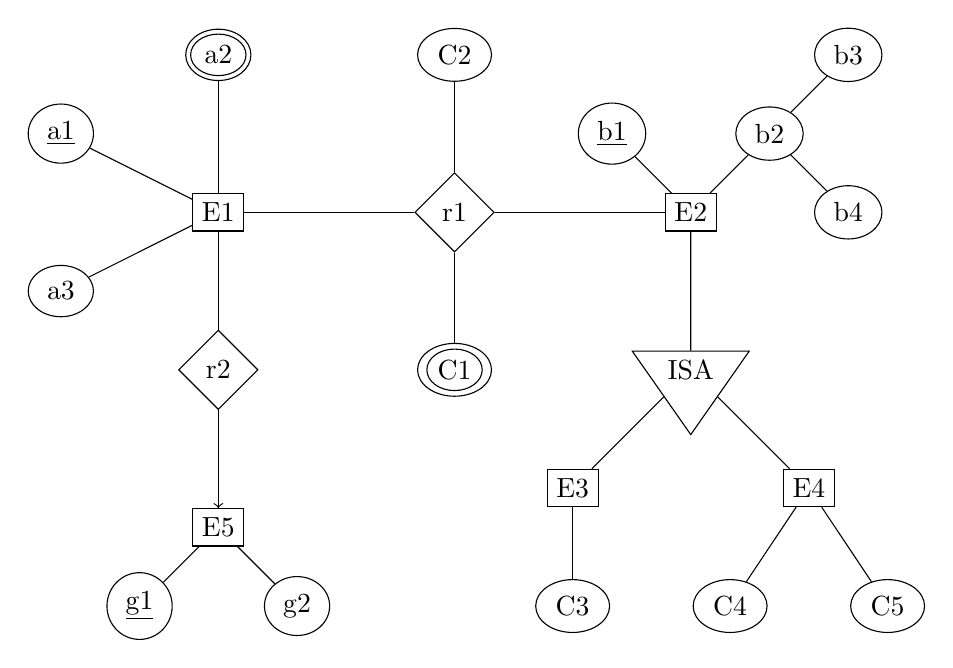
\begin{tikzpicture}
        \node(r1)at(0,0)[draw,diamond]{r1};
        \node(C2)at(0,2)[draw,ellipse]{C2};
        \node(C1)at(0,-2)[draw,ellipse]{C1};
        \node at(0,-2)[draw,ellipse,minimum width=2em,minimum height=1.5em]{};
        \node(E1)at(-3,0)[draw,rectangle]{E1};
        \node(a2)at(-3,2)[draw,ellipse]{a2};
        \node at(-3,2)[draw,ellipse,minimum width=2em,minimum height=1.5em]{};
        \node(a1)at(-5,1)[draw,ellipse]{\underline{a1}};
        \node(a3)at(-5,-1)[draw,ellipse]{a3};
        \node(r2)at(-3,-2)[draw,diamond]{r2};
        \node(E5)at(-3,-4)[draw,rectangle]{E5};
        \node(g1)at(-4,-5)[draw,ellipse]{\underline{g1}};
        \node(g2)at(-2,-5)[draw,ellipse]{g2};
        \node(E2)at(3,0)[draw,rectangle]{E2};
        \node(b1)at(2,1)[draw,ellipse]{\underline{b1}};
        \node(b2)at(4,1)[draw,ellipse]{b2};
        \node(b3)at(5,2)[draw,ellipse]{b3};
        \node(b4)at(5,0)[draw,ellipse]{b4};
        \node(ISA)at(3,-2)[draw,isosceles triangle,isosceles triangle apex angle=70,shape border rotate=-90]{ISA};
        \node(E3)at(1.5,-3.5)[draw,rectangle]{E3};
        \node(E4)at(4.5,-3.5)[draw,rectangle]{E4};
        \node(C3)at(1.5,-5)[draw,ellipse]{C3};
        \node(C4)at(3.5,-5)[draw,ellipse]{C4};
        \node(C5)at(5.5,-5)[draw,ellipse]{C5};
        \draw(E1)--(a2);
        \draw(E1)--(a1);
        \draw(E1)--(a3);
        \draw(E1)--(r2);
        \draw[->](r2)--(E5);
        \draw(g1)--(E5);
        \draw(g2)--(E5);
        \draw(E1)--(r1);
        \draw(C2)--(r1);
        \draw(C1)--(r1);
        \draw(r1)--(E2);
        \draw(E2)--(ISA);
        \draw(ISA)--(E3);
        \draw(E3)--(C3);
        \draw(E4)--(ISA);
        \draw(E4)--(C4);
        \draw(E4)--(C5);
        \draw(E2)--(b1);
        \draw(E2)--(b2);
        \draw(b2)--(b3);
        \draw(b2)--(b4);
    \end{tikzpicture}
\end{figure}
\section{(30 points) Consider the following relations in banking enterprise database, where the primary keys are underlined.}
\begin{description}
    \item[branch] (\underline{branch-name}, branch-district, assets)
    \item[employee] (\underline{employee-ID}, employee-name, branch-name, job-title)
    \item[loan] (\underline{loan-number}, branch-name, amount)
    \item[borrower] (\underline{customer-name}, loan-number, borrow-date)
    \item[customer] (\underline{customer-name}, customer-street, customer-city)
    \item[customerpoints] (\underline{customer-name}, scored-points) (注:客户积分表)
    \item[account] (\underline{account-number}, branch-name, balance)
    \item[depositor] (\underline{costomer-name}, \underline{account-number}, deposit-date) 
\end{description}\par
\subsection{(9 points) Use a SQL statement to define the relational table employee, in which [employee-ID] is the primary key, {employee-name} is the candidate key and not permitted to be null, and there exists referential integrity between the table employee and branch. It is also required that an employee's job -tile must be one of manager, teller, officer, or secretary.}
\subsection{(5 points) Give a SQL statement to find the customer' name who has one or more accounts at the branches located in Brooklyn district, and the total sum of the balances of his these accounts in Brooklyn is more thann \$10,000. It is required to list in alphabetic descending order the customer's name, and his total balances in the branches in Brooklyn.}
\subsection{(3 points) User1 needs to be able to read and update existing rows in employee. Define a SQL statement to give User1 only the privileges needed.}
\subsection{(3 points) Use a \textbf{relational algbra expression} to display the customer name, customer city, and points for \textbf{all} customers that have scored points.}
It is assumed that,
\begin{enumerate}[label=\alph*)]
    \item initially, each customer appearing in customerpoints has a positive points.
    \item not all customers in the table customer have scored points, also not all customers with scored points appear in customer.
\end{enumerate}
\subsection{(10 points) For the customers who appear in the table customer but have no scored points (i.e. not appear in the table customerpoints), use one or more SQL statements to add their names into customerpoints and set their scored points as 0.}
\section{(12 points) Consider the folowing relations and answer the Questions:}
\subsection{(6 points) The relation schema $R(U,F), U=(A,B,C,D,E)$. The functional dependencies set $F={A\rightarrow BC,CD\rightarrow E,B\rightarrow D,E\rightarrow A}$.}
\begin{enumerate}[label=\Alph*.]
    \item Compute $(B)^*$. List all the candidate keys of $R$.\quad(2 points)
    \item List all the candidate keys of $R$.\quad(4 points)
\end{enumerate}\par
\subsection{(6 points) The relation schema $R(U,F),U=(A,B,C,D,E)$, the functional dependencies set $F={A\rightarrow D,E\rightarrow D,D\rightarrow B,BC\rightarrow D,CD\rightarrow A}$. The Candiadate key of $R$ is ${C,E}$:}
\begin{enumerate}[label=\Alph*.]
    \item What is the highest normall form of $R$? Why?\quad(2 points)
    \item Give a lossless-join, dependency-preserving decomposition into 3NF of $R$.\quad(4 points)
\end{enumerate}\par
\section{(6 points) Consider the schema $R=(x,Y,W,Z,P,Q)$, and $F$, where\newline$F={XY\rightarrow WP,XW\rightarrow P,PQ\rightarrow Z,XY\rightarrow QZ}$ that holds on $R$.\quad(2 points)}
\subsection{Give the canonical cover of $F$.\quad(3 points)}
\subsection{Give a lossless-join, dependency-preserving decomposition into 3NF of $R$.\quad(3 points)}
\section{(6 points) Answer the following questions about the schema $R$.}
\subsection{$R={A,B,C,D,E,F},F={A\rightarrow B,C\rightarrow D,D\rightarrow E,E\rightarrow F,F\rightarrow C}$ that holds on $R$. List all the candidate keys of $R$.\quad(2 points)}
\subsection{$R={X,Y,Z,W,P},F={X\rightarrow YZ,ZW\rightarrow P,Y\rightarrow W,P\rightarrow X}$ that holds on $R$. What is the highest normal form of $R$? Why?\quad(4 points)}
\section{(11 points) Here are six schemas in the database "Company".}
\begin{description}
    \item[EMPLOYEE] (\underline{Esn}, Ename, BirthDate, LivingAddress, Sex, Salary, Mgr\_sn, DeptID)
    \item[DEPARTMENT] (\underline{DeptID}, DeptName, Mgr\_sn)
    \item[DEPT\_LOCATIONS]  (\underline{DeptID}, DeptLocation)
    \item[WORKS\_ON] (\underline{Esn}, \underline{PrjNo}, Hours)
    \item[PROJECT] (\underline{PrjNo}, PrjName, PLocation, DeptID)
    \item[DEPENDENT] (\underline{Esn}, \underline{DependentName}, Sex, BirthDate, Relationship)
\end{description}\par
Use SQL statements to implement the following operations:
\subsection{It is required that, the salary of an employee in a department should be lower than that of his manager in this department. Define this requirement as a constraint in the database.\quad(5 points)}
\subsection{Find out the department identity (i.e. DeptID) of each department, in which there are at least five emplyees, and calculate the number of the employees that have the salaries of more than \$5000 in this department.\quad(6 points)}
\newpage
\begin{center}
    \LARGE\sffamily 答案
\end{center}
\setcounter{section}{0}
\section{}
\subsection{view level, logical view, physical level}
\subsection{application programs do not depend on the physical schemas, and thus need not to be rewritten if the physical schemas change}
\section{phone可以使多值属性,两椭圆;children这是双线,其他联系双线单线都可。每处1分。}
\begin{figure}[H]
    \centering
    \begin{tikzpicture}
        \node(employee)at(0,0)[draw,rectangle]{employee};
        \node(salary)at(0,3)[draw,ellipse]{salary};
        \node(ssn)at(-2,3)[draw,ellipse]{\underline{ssn}};
        \node(phone)at(3,3)[draw,ellipse]{phone};
        \node(work)at(2,-3)[draw,diamond]{work};
        \node(manage)at(5,-3)[draw,diamond]{manage};
        \node(department)at(3.5,-6)[draw,rectangle]{department};
        \node(dno)at(7,-5)[draw,ellipse]{\underline{dno}};
        \node(dname)at(7,-6)[draw,ellipse]{dname};
        \node(budget)at(7,-7)[draw,ellipse]{budget};
        \node(has)at(-3,-3)[draw,diamond]{has};
        \node at(-3,-3)[draw,diamond,minimum width=3em,minimum height=3em]{};
        \node(children)at(-5,-5)[draw,rectangle]{children};
        \node at(-5,-5)[draw,rectangle,minimum width=4.25em,minimum height=1em]{};
        \node(name)at(-8,-4)[draw,ellipse]{\underline{name}};
        \node(age)at(-8,-5)[draw,ellipse]{age};
        \draw(employee)--(ssn);
        \draw(employee)--(salary);
        \draw(employee)--(phone);
        \draw[->](manage)edge[out=90,in=0,looseness=1](employee);
        \draw(employee)--(work);
        \draw[->](has)--(employee);
        \draw(children)edge[out=50,in=-150,looseness=0](has);
        \draw(children)edge[out=40,in=-140,looseness=0](has);
        \draw(name)--(children);
        \draw(age)--(children);
        \draw[->](work)--(department);
        \draw[->](manage)--(department);
        \draw(dno)--(department);
        \draw(dname)--(department);
        \draw(budget)--(department);
    \end{tikzpicture}
\end{figure}
\section{}
E1(\underline{a1},a3,g1)\par
E12(\underline{a1,a2})\par
E2(\underline{b1},b3,b4)\par
E3(\underline{b1},c3)\par
E4(\underline{b1},c4,c5)\par
E5(\underline{g1},g2)\par
R1(\underline{a1,b1},c2)\par
R2(\underline{a1,b1,c1})\par
\section{}
\subsection{4个完整性约束,每个1分。}
\begin{verbatim}
create table employee(
    employee-ID	     integer,
    employee-name    varch(50), /*也可以采用其它长度的varch, char类型
    branch-name	     varch(50),
    job-title        varch(50),
    primary key (employee-ID),
    unique (empolyee-name),
    foreign key (branch-name) references branch,
    check (job-title in ('manager', 'teller', 'officer', 'secretary'))
)
\end{verbatim}
\subsection{\texttt{group by}和\texttt{having}子句占2分,其余部分3分。}
\begin{verbatim}
    Select customer-name, sum(balance)
    From branch Natual Join account Natual join depositor
    Where branch-district=Brooklyn
    Group by customer-name
        Having sum(balance)>10,000
    Order by customer-name desc
\end{verbatim}
\subsection{\texttt{grant select, update on employee to User1}}
\subsection{如果没有写出左外连接符号、只写出自然连接符号,扣1分。}
$\Pi$\textsubscript{customer-name, customer-city, points}(customerpoints left-touter-join 符号 customer)
\subsection{2个句子各5分。}
\begin{verbatim}
    Select customer-name into Temp
    From customer
    Where customer-name not in ( select customer-name
                                 from customerpoints
                               )
    Insert into customerpoints
            Select customer-name, 0
            From Temp
\end{verbatim}
\section{}
\subsection{}
\begin{enumerate}[label=\Alph*.]
    \item $BD$
    \item $A,BC,CD,E$
\end{enumerate}
\subsection{}
\begin{enumerate}[label=\Alph*.]
    \item 1NF
    \item 本身就是最小函数依赖集。$R1(ED),R2(BCD),R3(CDA),R4(CE)$
\end{enumerate}
\section{${XY\rightarrow WQ,XW\rightarrow P,PQ\rightarrow Z}$}
\section{}
\subsection{$AC,AD,AE,AF$}
\subsection{$3NF$}
\section{}
\subsection{}
\begin{verbatim}
    create assertion Salary_constraint
        check ( not exists
            ( select *
              from EMPLOYEE as E, EMPLOYEE as M, DEPARTMENT as D
              where E.salary>M.salary
                AND E.DeptID=D.DeptID
                AND D.Mgr_sn=M.Esn
            )
\end{verbatim}
\subsection{}
\begin{verbatim}
    select  DeptID, count(*)
    from    DEPARTMENT as D, EMPLOYEE as E
    where   D.DeptID in ( select E.DeptID
                          from EMPLOYEE
                          group by E.DeptID
                          having count(*)>5
                        )
\end{verbatim}
\end{document}
